\chapter{RTKGPS}
\section{Error sources}
In order to get high accuracy in the position estimation the different error sources must be identified and removed if possible. This section will identify some of the most significant error sources that can affect the \gls{gps} signal, and how to remove or mitigate them in the estimation.
\subsection{Clock error}
There is drift in both the satellite clock and the receiver clock. The atomic clock in the satellites makes the clock drift negligible from the user perspective. The receiver clock tend to drift, and if not taken into account will cause large deviations in the position estimate from the true position. This error is remove by including a fourth satellite in the position computation. The satellite clock error is given in the satellite message. 

\subsection{Ionospheric and tropospheric delays}
When the \gls{gps} signals travel though the atmosphere there will be a delay caused by the different atmospheric layers.
\subsubsection{Ionospheric delay}
Gas molecules in the ionosphere becomes ionized by the ultraviolet rays that is emitted by the sun, which release free electrons. These electron can influence electromagnetic wave propagation, such as GNSS signals. The delay that the signal get from the ionosphere may cause a error the the order of $1-10 $meters. The error can be mitigated by using a double frequency receiver, or by applying a mathematical model to estimate the delay. Both those methods are with a single receiver, however by including a second receiver the GNSS solution system can assume that both receiver receive signal in the same epoch, which means that the signals have experienced the same delay. This will be further explain in section \ref{ss: Error mitigation DGPS}.

\subsubsection{Tropospheric delay}
The tropospheric delay is a function of the local temperature, pressure and relative humidity. The delay can vary from $2.4$ meters to $25$ meters depending on the elevation angle of the satellites. The error can be mitigated by applying a mathematical model to estimate the tropospheric delay, or by using a elevation mask can remove all satellites with a elevation angle bellow a certain threshold. Error caused by tropospheric delay can be removed in the same manners as ionospheric delay when using two or more receivers. This will be further explain in section \ref{ss: Error mitigation DGPS}.

\subsection{Ephemeris errors}
A satellite is not able to perfectly follow a given orbit, therefore there will be a deviation between satellite position given to the receiver and the true position of the satellite. This is called the ephemeris error. The true position of a satellite is monitored and corrected by the owner of the \gls{gnss} constellation, but error between each correction can be expected.
\subsection{Multipath}
One of the primary source of error in in a GNSS receiver is multipath. Multipath happens when the satellite signal is reflected by a nearby surface before if reach the \gls{gnss} antenna. The delay introduced in the signal can make the receiver believe that its position is several meters away form its true position. The easiest way to mitigated multipath is to place the antenna at a location with open skies, and no tall structures nearby.
\section{Differential GPS}
\acrfull{dgps} consist of at least two receivers, where one is called a base station and the rest rovers. For simplicity only two receiver is used in this section. The two receivers are within range of a communication channel over which they are communicating, as shown in figure \ref{figure:DGPS}. The base station has a known position, and the rover estimate the baseline from itself to the base station.

In this project work only carrier phase measurements will be considered for position estimation method.
The problem with precise relative positioning with carrier phase measurement is problem of estimation of integer ambiguities.

\begin{figure}[H]
	\centering
		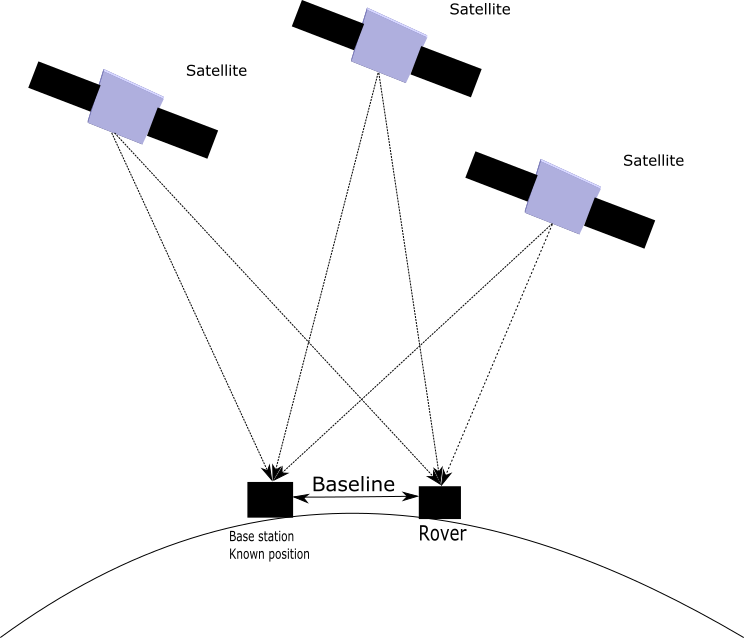
\includegraphics[width=0.7\textwidth]{figs/DGPS.png}
		\caption{Concept figure of \acrfull{dgps}}
		\label{figure:DGPS}
\end{figure}
\subsection{Error mitigation in DGPS} \label{ss: Error mitigation DGPS}
In \gls{dgps} the rover considers that both the rover and base station receive \gls{gps} signal that has experienced the same delay. Thus the rover can remove all error sources that is correlated with the base station. This assumption holds given that the baseline is not to long. For longer baseline other methods must be applied to correct for atmospheric delay. \gls{dgps} error mitigation do not include multipath. Multipath is an uncorrelated error, and thus must be corrected locally by both the rover and base station.


\section{Real time kinematic GPS}\label{ss:rtk-gps}
\acrfull{rtk-gps} is a variant of \gls{dgps} where raw data is sent from the base station to the rover, where the distance between them is calculated in real time.
The distance between the rover and base station is referred to as a baseline. The difficulty with \gls{rtk-gps} is the ability to estimate the integer ambiguities while the rover is moving. A fixed integer ambiguities solution results in a accurate baseline estimate.

\gls{rtk-gps} can either provide a kinematic setting or a moving baseline setting. The difference between the two is that in kinematic the base station has a known stationary position, while in moving baseline the base station position is unknown and allowed to move. The unknown base station position is calculated with a single receiver, with the accuracy that entails. Therefore the \gls{rtk-gps} system with a moving baseline configuration can never have better global accuracy then what it will get with a single receiver. The advantage with the moving baseline configuration is that \gls{rtk-gps} can be used to find the relative position between two dynamical system using \gls{gnss} in real time. This will be the case in automatic ship landing system, where the base station is on a ship, thus must be allowed to move. The advantage with kinematic mode is that it can give a more accurate position estimate, where the relative position of the rover can be given in either the \gls{ned} or \gls{enu} frame.
\cleardoublepage